
\documentclass[10pt,a4paper]{article}
\usepackage[T1]{fontenc}
\usepackage{tikz}
\usepackage[margin=1cm]{geometry}
\begin{document}

\section*{Final Binary Tree:}
This document presents the final binary tree generated through the user-driven node insertion process. The binary tree structure is designed to start from a root node and grows as new nodes are inserted based on user input. The following sections detail the algorithm and the visualization of the tree.

\subsection*{Tree Construction Process:}
The binary tree was constructed using the following steps:
\begin{enumerate}
    \item \textbf{Insertion of Root Node:} The process began by inserting the root node, which is the starting point of the tree.
    \item \textbf{Adding Child Nodes:} For each subsequent node, the user was prompted to specify the parent node and whether the new node should be placed on the left or right.
    \item \textbf{Recursive Structure:} The tree maintains a recursive structure, where each node can have up to two children (left and right). The final tree reflects all user inputs.
\end{enumerate}

\vspace{1cm}

\begin{center}
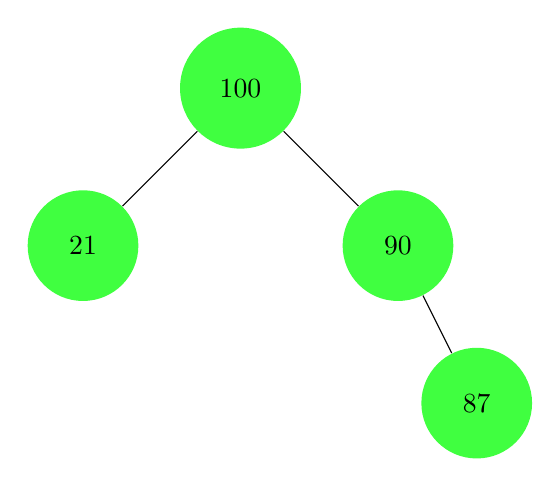
\begin{tikzpicture}[level distance=20mm]
    \tikzstyle{every node}=[fill=green!75,circle,inner sep=10pt, minimum size=8mm]
    \tikzstyle{level 1}=[sibling distance=40mm, set style={{every node}+=[fill=green!75]}]
    \tikzstyle{level 2}=[sibling distance=20mm, set style={{every node}+=[fill=green!75]}]
    \tikzstyle{level 3}=[sibling distance=10mm, set style={{every node}+=[fill=green!75]}]
    \tikzstyle{level 4}=[sibling distance=5mm, set style={{every node}+=[fill=green!75]}]
    \node {100} child {node {21} } child {node {90} child[fill=none] {edge from parent[draw=none]} child {node {87} }};

\end{tikzpicture}
\end{center}

\subsection*{Understanding the Visualization:}
The tree diagram above visually represents the binary tree. Each circle represents a node, and the connections between them represent the parent-child relationships. The root node is the topmost circle, and all other nodes are connected below it. The position of each node (left or right) corresponds to its relation to the parent node, as determined by the user's input during the tree construction process.

\end{document}
